\documentclass{report}
\usepackage[T1]{fontenc} % Fontes T1
\usepackage[utf8]{inputenc} % Input UTF8
\usepackage{csquotes}
\usepackage[portuguese]{babel} %Usar língua portuguesa
\usepackage{blindtext} % Gerar texto automaticamente
\usepackage[printonlyused]{acronym}
\usepackage{hyperref} % para autoref
\usepackage{graphicx}
\usepackage{float}


\begin{document}
%%
% Definições
%
\def\titulo{Projeto Redes}
\def\data{Dezembro 2021}
\def\autores{Pompeu Costa(103294), Guilherme Craveiro(103574)}
\def\logotipo{ua.pdf}
%
%%%%%% CAPA %%%%%%
\begin{titlepage}

\begin{center}
%
\vspace*{50mm}
%
{\Huge \titulo}\\ 
%
\vspace{10mm}
%
%
\vspace{10mm}
%
{\LARGE \autores}\\ 
%
\vspace{30mm}
%
\begin{figure}[h]
\center
\includegraphics{\logotipo}
\end{figure}
%
\vspace{30mm}
\end{center}
\end{titlepage}

%%%%%%%%%%%%%%%%%%%%%%%%%%%%%%%
\clearpage
\pagenumbering{arabic}

%%%%%%%%%%%%%%%%%%%%%%%%%%%%%%%%
\begin{center}
\begin{figure}
    \centering
    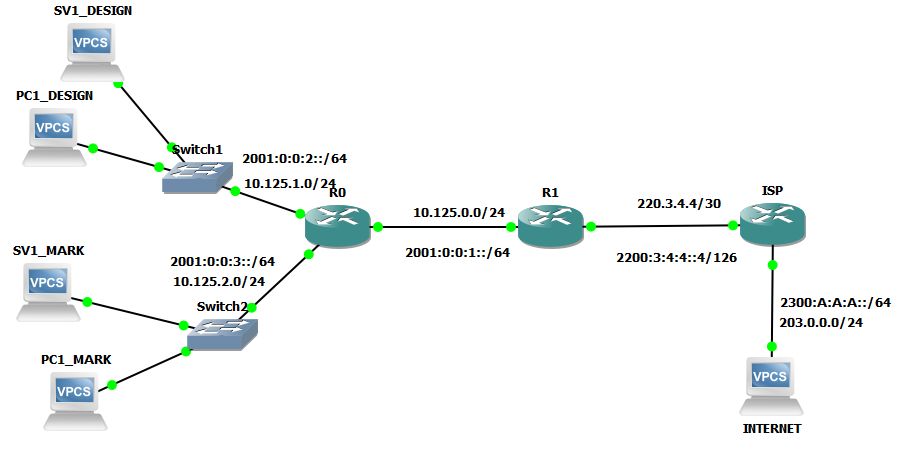
\includegraphics[scale=0.65]{network.png}
\end{figure}
\end{center}
\begin{center}
    
\end{center}
\begin{tabular}{|c|c|c|c|}
    \hline
    Rede & IPv4 Público & IPv4 Privado & IPv6 \\
    \hline
    R1 -> R0 & -------- & 10.125.0.0/24 & ???? \\
    \hline
    DESIGN & 200.132.135.128/26 & 10.125.1.0/24 & ???? \\
    & & GW- 10.125.1.1 & \\
    \hline
    MARKETING & 200.132.135.192/27 & 10.125.2.0/24 & ???? \\
    & & GW- 10.125.2.1 & \\
    \hline
    R1 -> ISP & 220.3.4.4/30 & -------- & ???? \\
    \hline
    ISP -> INTERNET & 203.0.0.0/24 & -------- & ????\\
    \hline
\end{tabular}

\begin{center}
\begin{figure}
    \centering
    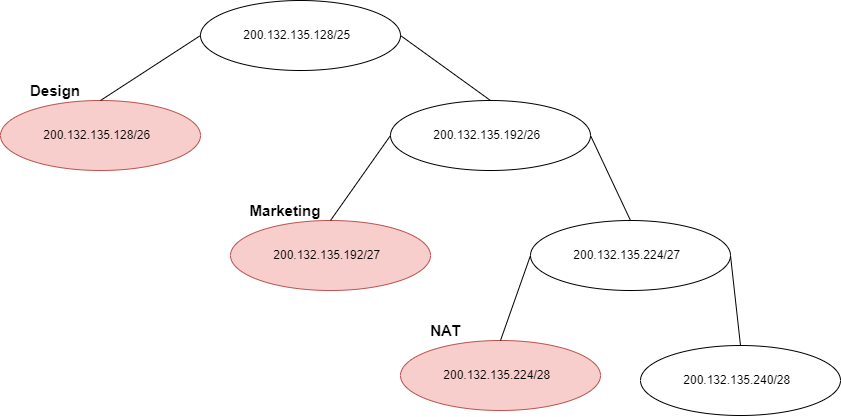
\includegraphics[scale=0.5]{IPsPublicosDiagrama.png}
\end{figure}    
\end{center}
\end{document}
